%% ----------------------------------------------------------------------------
%\begin{frame}{Agenda}
%\begin{enumerate}
%	\setcounter{enumi}{3}
%	\item Ambiente de Teste e Resultados Preliminares
%	\bigskip
%	\begin{itemize}
%		\item Avalia��es: objetiva e subjetiva
%		\bigskip
%		\item Perfil dos volunt�rios 
%		\bigskip
%		\item Resultados preliminares com o AGR
%	\end{itemize}
%\end{enumerate}
%\end{frame}

%%%%%%%%%%%%%%%%%%%%%%%%%%%%%%%%
\subsection{Testes}
\begin{frame}{Participantes}

\begin{itemize}
    \item 20 participantes: Estudantes de gradua��o ou p�s-gradua��o da UFPA
    % \item Exig�ncia m�nima: familiaridade com os \textit{websites} escolhidos no teste 
    \item Termo de consentimento
\end{itemize}

\end{frame}

\begin{frame}{Dwell Time e eViacam}
    \begin{figure}
        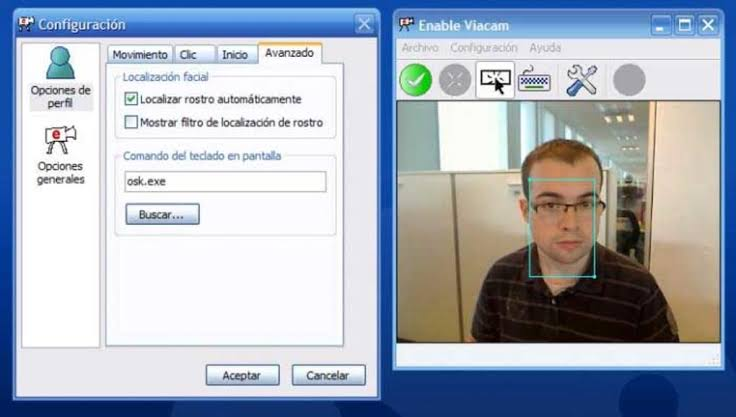
\includegraphics[width=0.9\linewidth]{Figures/eviacam}
    \end{figure}
\end{frame}

\begin{frame}{Ambiente de Teste}
\begin{itemize}
\item Ambiente bem iluminado
\item Cadeira de frente para um \textit{laptop} equipado com {webcam}
% \item Dois m�todos de clique: Baseado em sopro e \textit{dwell time}
\item (\textit{Dwell time + Eviacam}) X (Sopro + Giroscopio/Aceler�metro)
\end{itemize}
\end{frame}


\begin{frame}{Tarefas}
    \begin{itemize}
        \item Testes realizados no \textit{website} G1
        \item[--] Dificuldade na utiliza��o para PCD
    \end{itemize}
	\begin{figure}
		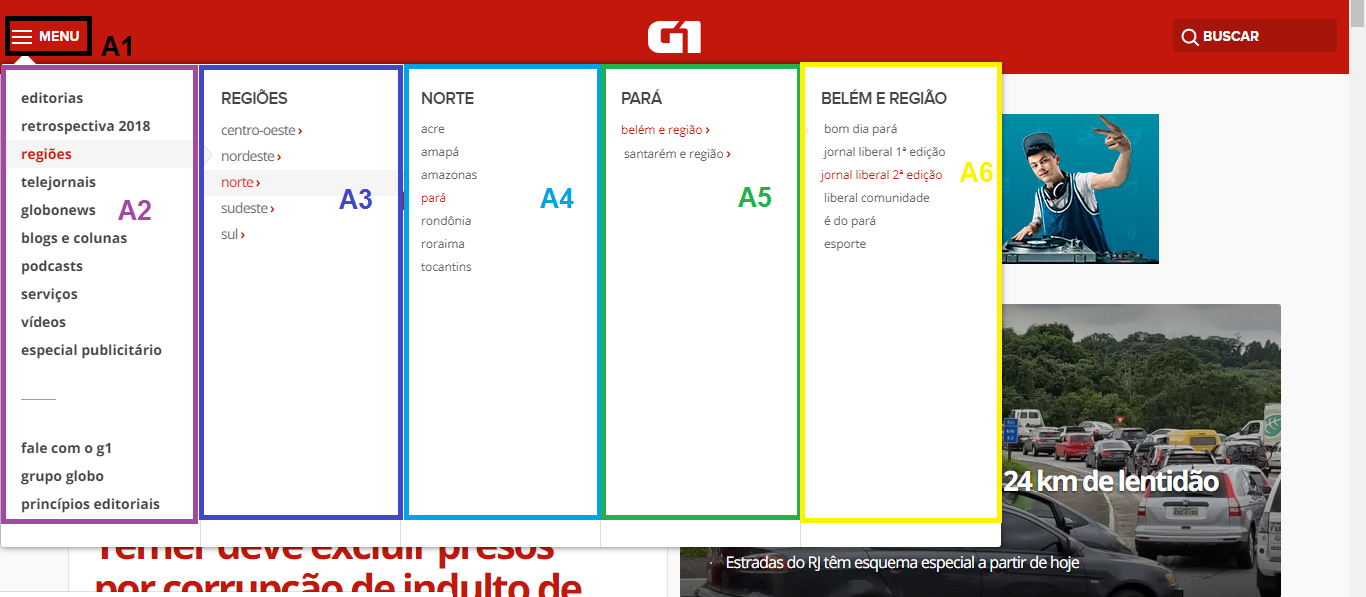
\includegraphics[width=\linewidth]{Figures/g1_areas}
        \caption{�reas de interesse destacadas pelos ret�ngulos A1, A2, etc.}
	\end{figure}

\end{frame}



\begin{frame}{Avalia��es}
\begin{itemize}
\item \textbf{Quantitativa}: Tempo de execu��o e erros de cliques   
\item \textbf{Qualitativa}: Question�rio objetivo com 6 quest�es
\item \textbf{Subjetiva}: Pergunta subjetiva sobre o dispositivo de sopro 
\end{itemize}

\end{frame}





\subsection{Resultados Quantitativos}
\begin{frame}{Resultados Quantitativos [1/2]}
	\centering
	\begin{figure}
		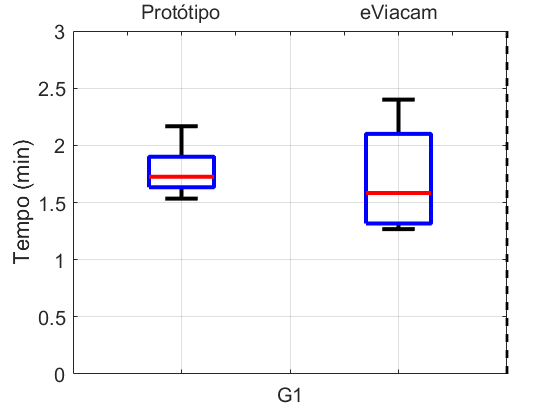
\includegraphics[width=0.8\textwidth]{Figures/tempo_g1}
		\caption{Tempo de execu��o das tarefa.}
	\end{figure}
\end{frame}

\begin{frame}{Resultados Quantitativos [2/2]}
	\centering
	\begin{figure}
		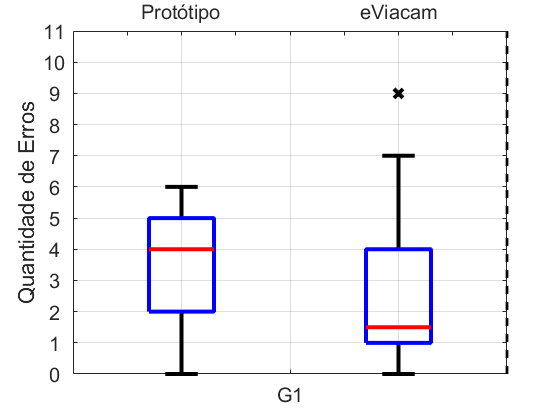
\includegraphics[width=0.8\textwidth]{Figures/erros_g1}
		\caption{Erros de cliques cometidos.}
	\end{figure}
\end{frame}

% \begin{frame}{Resultados Quantitativos [3/3]}
% 	\begin{figure}
	
% 	\makebox[\linewidth]{\parbox{12cm}{  %{\lipsum}}
% 		\subfloat[Dwell time.]{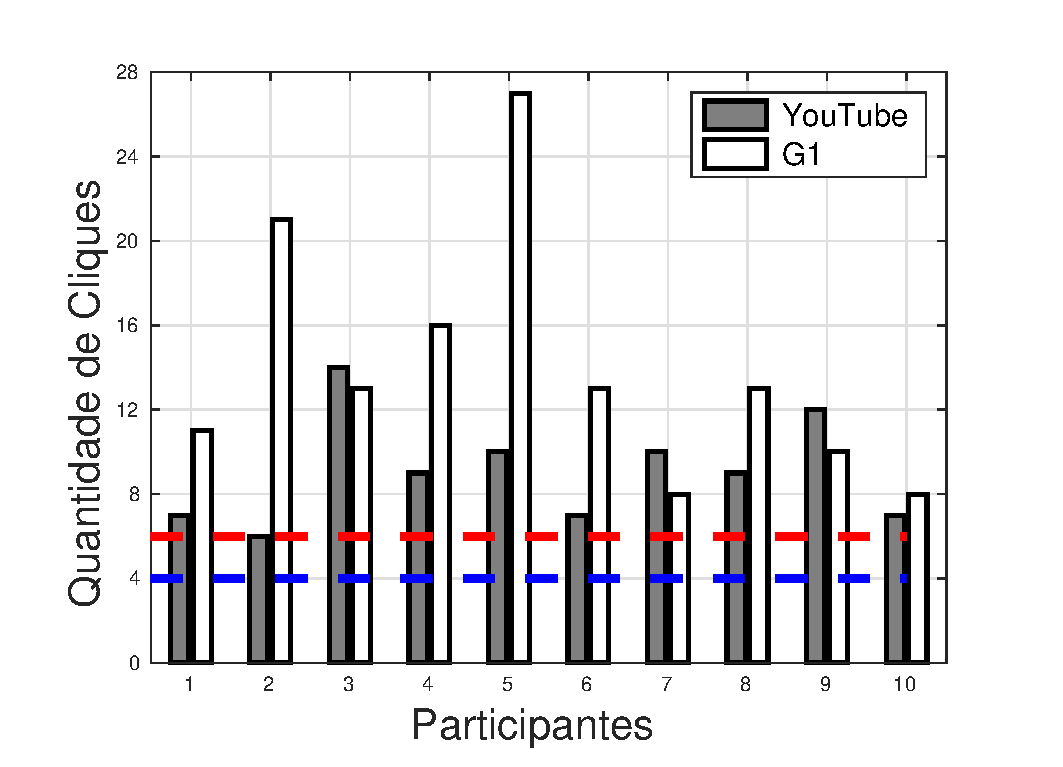
\includegraphics[width=0.5\linewidth]{Figures/DwellClicks}} \quad
% 		\subfloat[Sopro.]{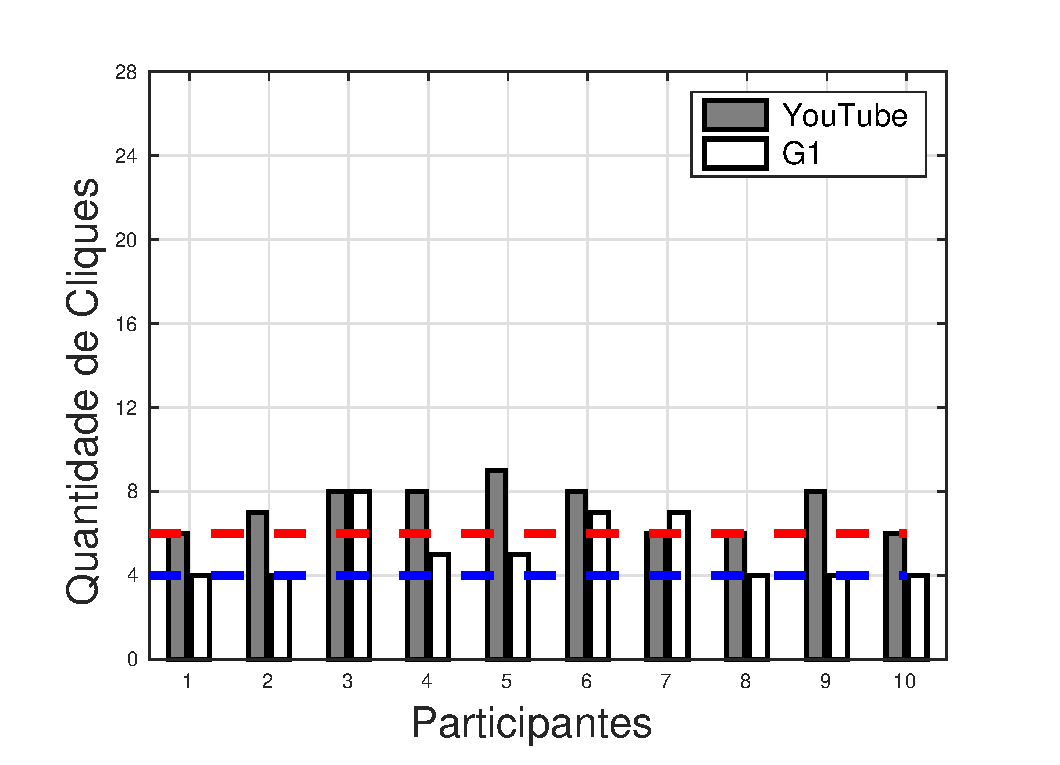
\includegraphics[width=0.5\linewidth]{Figures/PuffClicks}}
% }}
% 	\end{figure}

% \end{frame}

\subsection{Resultados Qualitativos}
\begin{frame}{Question�rio Objetivo}
\begin{table}[!t]
\centering
\begin{tabular}{cc|ll}
	\hline
	\hline
	~ & \textbf{Pergunta} & \multicolumn{2}{c}{\textbf{Resposta}} \\
	\hline \textbf{1} & Experi�ncia de uso & 1 -- insuficiente & 5 -- excelente \\
	\textbf{2} & Tempo & 1 -- lento & 5 --  r�pido \\
	\textbf{3} & Precis�o& 1 -- insuficiente & 5 -- excelente \\
	\textbf{4} & Esfor�o cognitivo& 1 -- alto & 5 -- baixo\\
	\textbf{5} & Esfor�o f�sico & 1 -- alto & 5 --  baixo\\
	\textbf{6} & Concentra��o & 1 -- mais no clique & 5 -- mais na tarefa \\
	\hline
	\hline
\end{tabular}
\end{table}

\begin{minipage}{.1\textwidth} 

\end{minipage}
\noindent\hspace{0.28\linewidth}\begin{minipage}{.7\textwidth} 
\begin{itemize}
\item[\textcolor{black}{$\blacksquare$}]   Escala Likert
\begin{itemize}
\item[\textcolor{red}{$\blacksquare$}] 1 --- Muito Ruim 
\item[\textcolor{orange}{$\blacksquare$}] 2 --- Ruim       
\item[\textcolor{yellow}{$\blacksquare$}]   3 --- Regular    
\item[\textcolor{erick}{$\blacksquare$}]   4 --- Bom        
\item[\textcolor{suzane}{$\blacksquare$}] 5 --- Muito Bom  
\end{itemize}
\end{itemize}
\end{minipage}
\begin{minipage}{.1\textwidth}

\end{minipage}

\end{frame}


\begin{frame}{Question�rio Objetivo - An�lise}
	
	% \begin{figure}
	% 	\begin{minipage}{.85\textwidth}
	% 	\subfloat{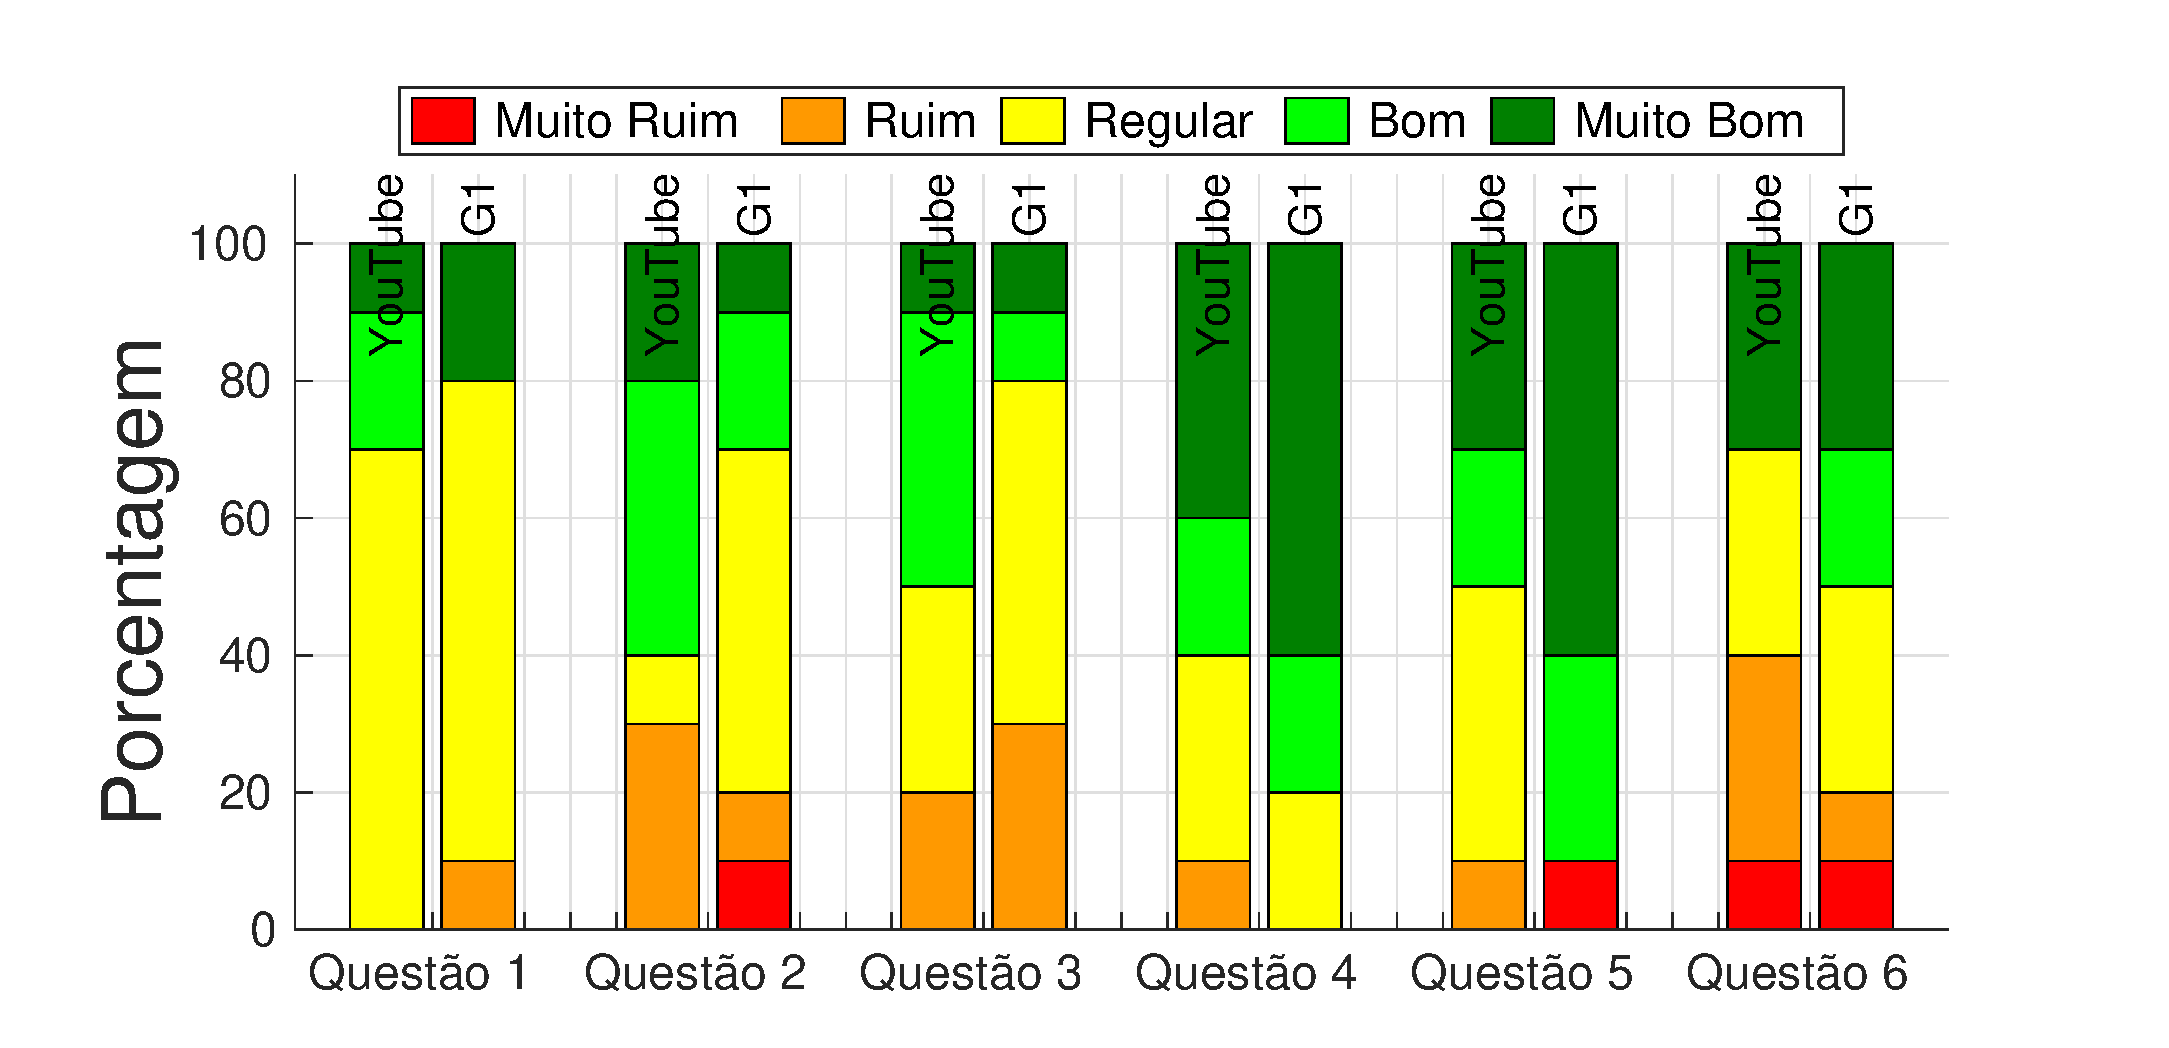
\includegraphics[width=0.95\linewidth]{Figures/DwellQuestions}}\\
	% 	\end{minipage}
	% 	\begin{minipage}{.1\textwidth}
	% 	\textit{Dwell time}
	% 	\end{minipage}

	% 	\begin{minipage}{.85\textwidth}
	% 	\subfloat{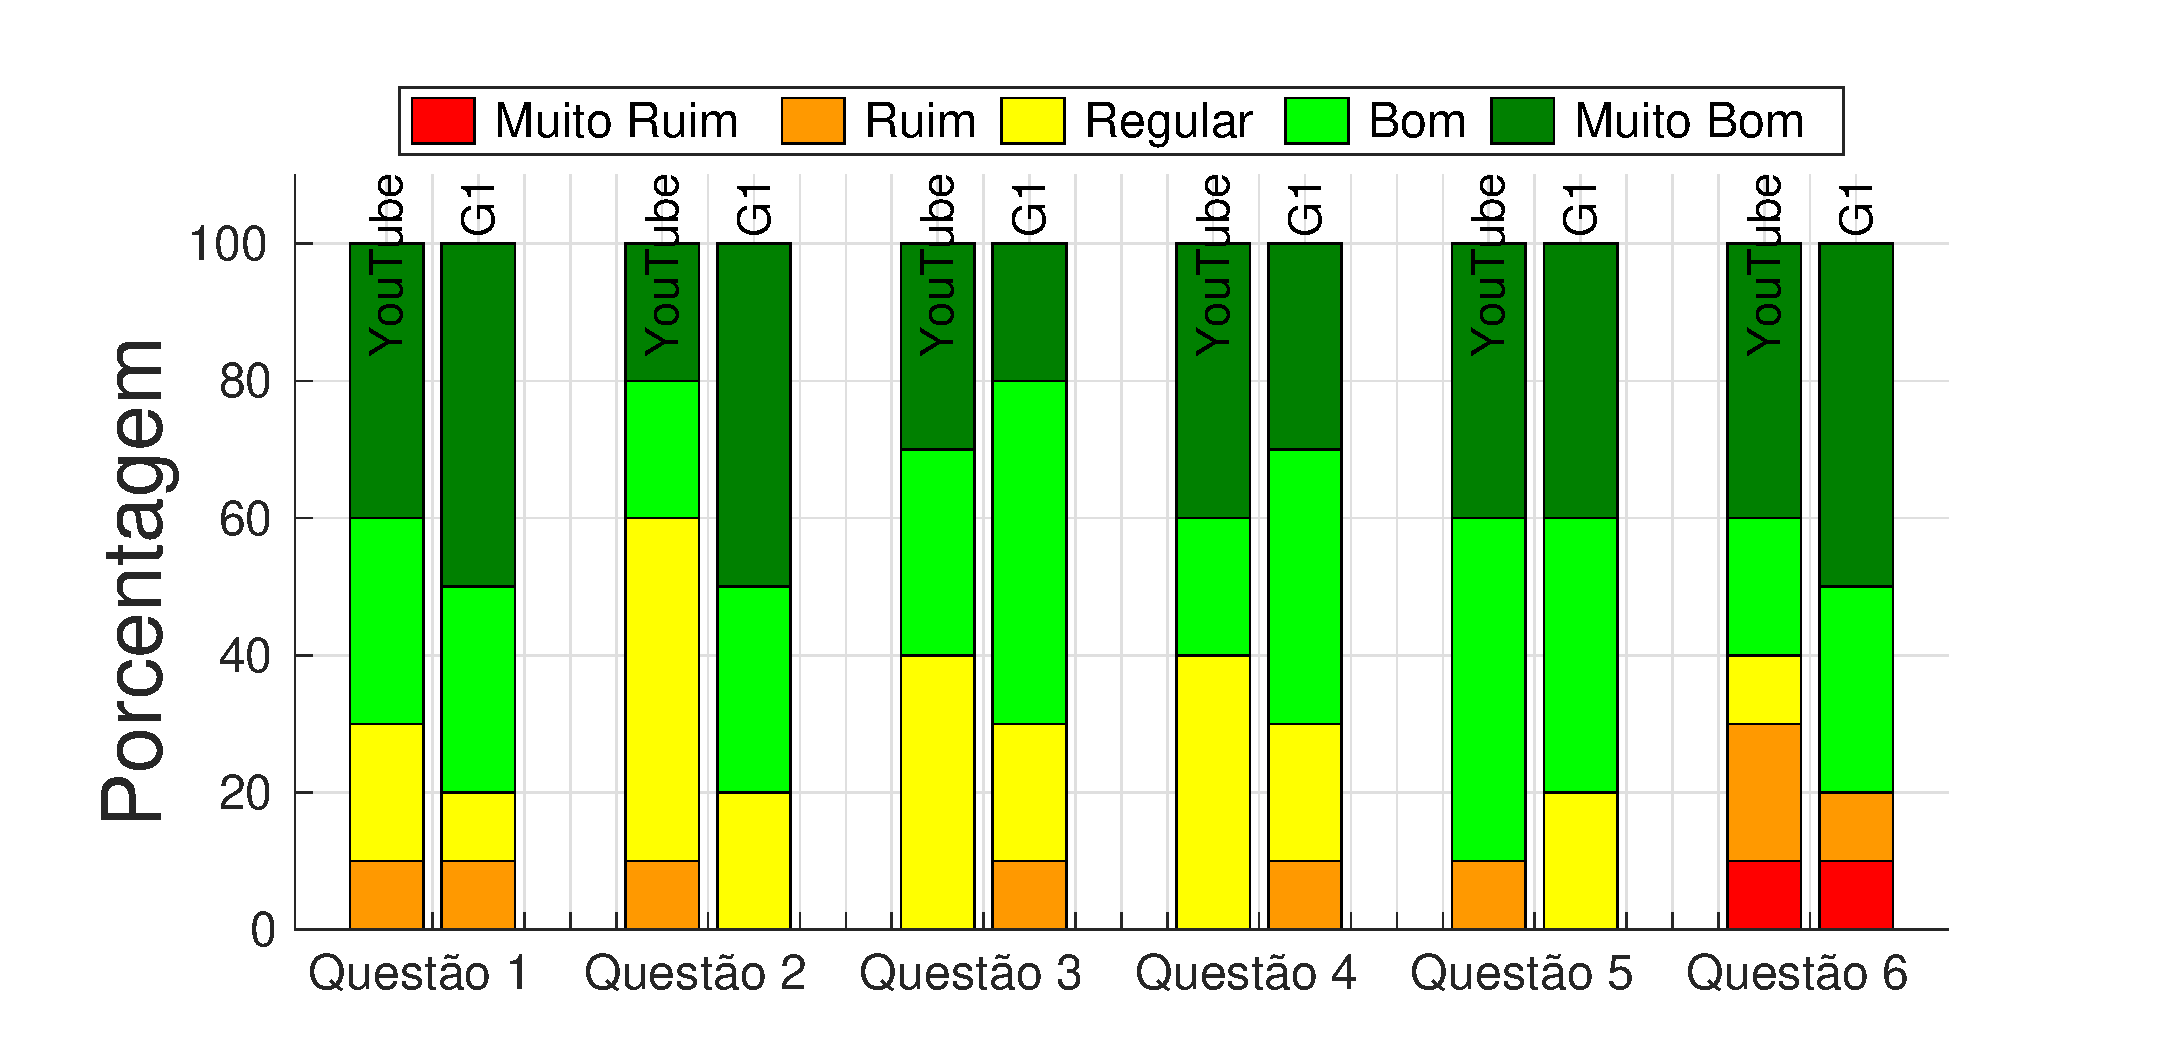
\includegraphics[width=0.95\linewidth]{Figures/PuffQuestions}}
	% 	\end{minipage}
	% 	\begin{minipage}{.1\textwidth}
	% 	Sopro
	% 	\end{minipage}
	% \end{figure}

    \begin{figure}
        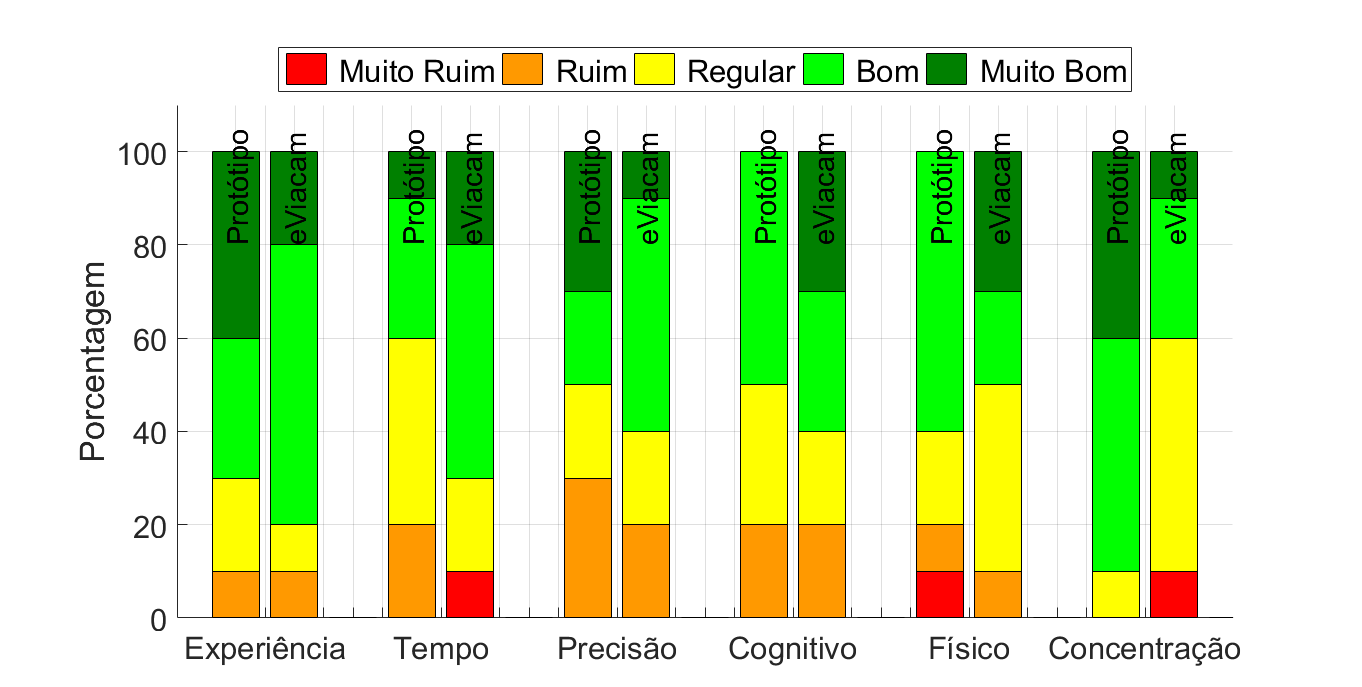
\includegraphics[width=\linewidth]{Figures/likert}
        \caption{Escala Likert para prot�tipo e eViacam}
    \end{figure}

\end{frame}

% \begin{frame}{An�lise dos Resultados}
%     \begin{itemize}
        % \item 
% \end{frame}

\subsection{Quest�o Subjetiva}
\begin{frame}{Discuss�o Sobre a Quest�o Subjetiva}

\begin{center}
\textbf{``Com base na sua experi�ncia de uso, que sugest�es voc� daria para melhoria do dispositivo?''}
\end{center}

\begin{itemize}
\item Cliques involunt�rios
\item Centraliza��o do cursor
\item Substitui��o do \textit{headset}
\item Sensibilidade ajust�vel
\item \textit{Feedback} visual a fim de mostrar o n�vel de sensibilidade
\end{itemize}

\end{frame}
